\documentclass[a4paper,11pt]{article}
\usepackage{graphicx}

\begin{document}

\begin{flushright}

\vspace{1.1cm}

%Put ISR Title
{\bf\Huge Problem Set 2}

\rule{0.25\linewidth}{0.5pt}

\vspace{0.5cm}
%Put Authors
Justin Ely
\linebreak
\newline
%Put Author's affiliations
\footnotesize{AST622 University of Maryland College Park, MD\\}
\vspace{0.5cm}
% Date here below
08 March, 2012
\end{flushright}

\noindent\rule{\linewidth}{1.0pt}
\section*{1) Angular and Luminosity Distance}
\subsection*{a] Angular Diameter Distance}

\begin{eqnarray}
d_A=\frac{r(x)}{1+z}  \\
r(x)=\frac{sinh(\sqrt{\Omega_k}H_0 x)}{H_0 \sqrt{\|{\Omega_k}\|}}
\end{eqnarray}


In Figure 1 we see a plot of angular diameter distance vs redshift for a matter dominated universe with negative curvature.  From the plot we see that the angular diameter distance decreases continuously as z increases.  This is different from universes with positive curvature, where the angular diameter distance will decrease until some minimum, and then begin to increase.  


\subsection*{b] Magnitude-Redshift Diagram}
\begin{eqnarray}
m-M=5log(d_L)+25 \\
d_L=\frac{2c}{H_0 \Omega_0^2}(\Omega_0 z +(\Omega_0 -z)[-1+(\Omega_0 z+1)^{\frac{1}{2}}])
\end{eqnarray}

Figure 2 shows the magnitude-redshift diagram for various universes.  This plot shows that the distance modulus increases with increasing redshift, but at a slower pace with a closed universe.


\section*{2) Thermal History}
\subsection*{a] Entropy}
Entropy conservation is a better approximation than energy conservation because while the number density per unit volume for radiation remains the same as the universe expands, the energy of the photons decreases with the expansion.  In contrast, entropy remains constant per unit volume.  


\begin{eqnarray}
T=\frac{\bar{g}_0}{\bar{g}}^{1/3} \frac{T_\gamma}{a} \\
H(t)=\frac{\dot{a}}{a}=\frac{8\pi G}{3}\rho
\end{eqnarray}

Combines into:
\begin{equation}
\frac{\dot{T}}{T}=(\frac{8\pi G a_r}{3c^2})^{1/2}\frac{g_t^{1/2}}{(1+\frac{1}{3}\frac{T}{\bar{g}(T)}\frac{d\bar{g}(T)}{dT})}T^2 
\end{equation}


\subsection*{b] Relic Abundance}
Using the equation from the notes:
\begin{equation}
F=12(\frac{g_x (1+\delta_f)}{g_f^{1/2}})(\frac{m_xc^2}{1GeV})(\frac{1.24x10^9}{\mu c^2})^2
\end{equation}

Leads to :

\begin{equation}
F=12(\frac{2}{\sqrt{15}})(\frac{m_xc^2}{1GeV})(\frac{1.24x10^9}{.135 GeV})^2=5.71x10^{20}
\end{equation}

Interactively solving:
\begin{equation}
\chi_f^{(2)}=log(F)+\frac{1}{2}log(log(F))=49.73  \\
\end{equation}

\begin{equation}
\Omega_xh^2=\chi_f\frac{\sqrt{g_f}}{\bar{g_f}}(1.8x10^{-14})=8.4x10^{-14} \\
\end{equation}

This relic abundance is so small because the cross section for baryon annihilation is very large, which means that most of the baryons have ample time to annihilate before the universe can expand enough for freezout to happen.  For WIMPS, with a much smaller cross section, freezout happens before a significant fraction of the particles can annihilate.

\section*{3) Primordial Black Holes}
\subsection*{a] Mass in Particle Horizon}
Using an equation from the notes:
\begin{equation}
a=(2H_o \sqrt{\Omega_R}t)^{1/2}
\end{equation}

Using $\Omega_R=\frac{\rho_R}{\rho_{crit}}$, $a=(1+z)^{-1}$, and $\rho=mass/volume$:
\begin{equation}
m_{hor}=(\frac{2}{3})\frac{\rho_{crit} \pi r_h^{3}}{H_o}(\frac{(1+z)^{-2}}{t})
\end{equation}


\subsection*{b] Horizon Mass vs Black Hole}
Using the particle horizon, $r_{hor}=4.6x10^{10}ly=4.35x10^{28}cm$, and mean cosmic density, $\rho=5x10^{-30}g/cm^3$, we can compare the mass of the universe to the Jeans mass and the mass of a black hole.  We can see below that the mean density of the universe within the particle horizon is a factor of 5 higher than the Jeans mass and the criteria for a black hole. 
\begin{equation}
M_{hor}=\rho \frac{4}{3}\pi r_{hor}^3=1.6x10^{57}
\end{equation}
\begin{equation}
M_j=\frac{4\pi}{3}\frac{c}{6}^3(G^{-3/2})(\rho^{-1/2})=5.25x10^{52}
\end{equation}
\begin{equation}
M_{bh}=\frac{r c^2}{2G}=2.93x10^{52}
\end{equation}

\section*{A) Figures}

\begin{figure}[h!]
\begin{center}
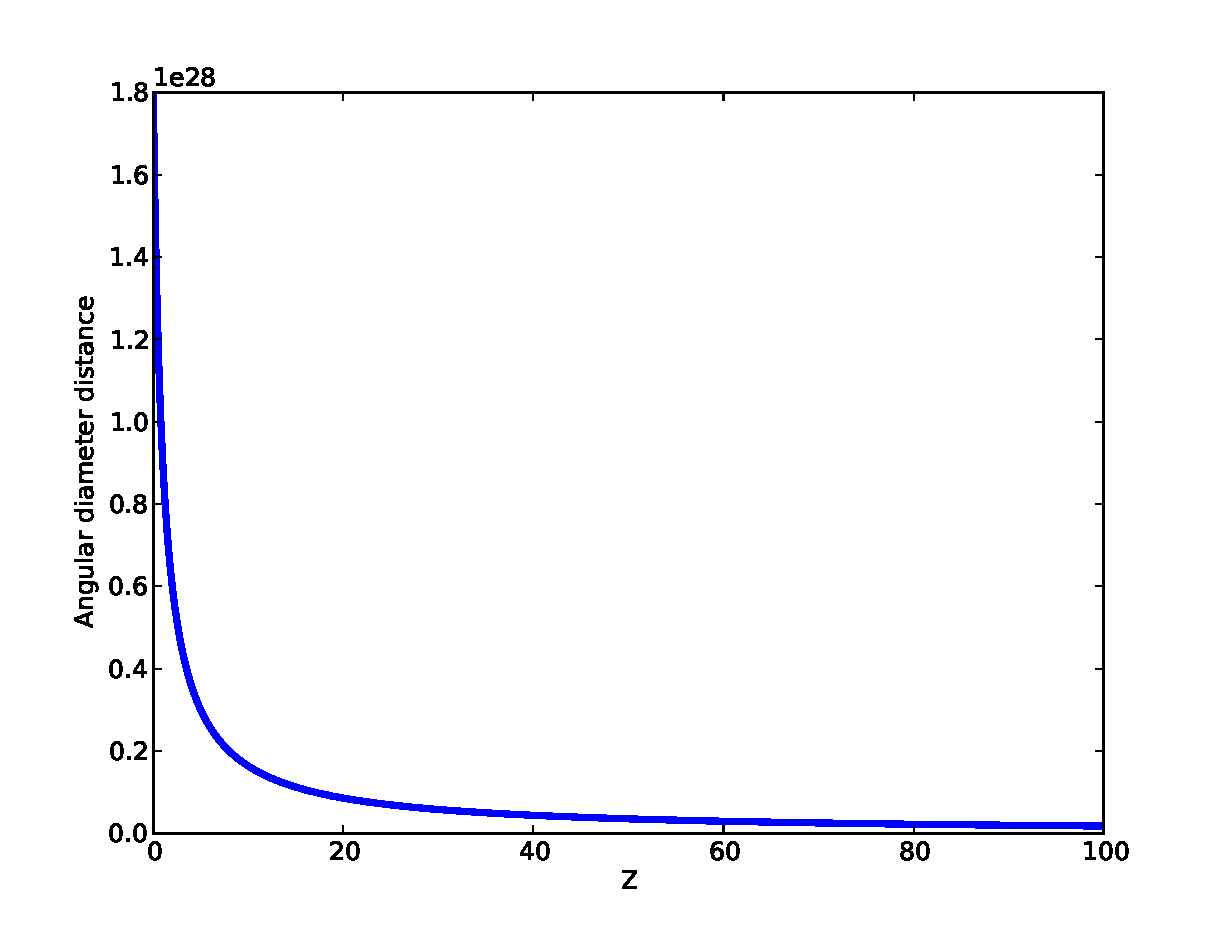
\includegraphics[scale=.6]{plot_1.pdf}
\caption{Angular diameter distance as a function of redshift for a matter dominated universe with negative curvature.}
\end{center}
\end{figure}

\begin{figure}[h!]
\begin{center}
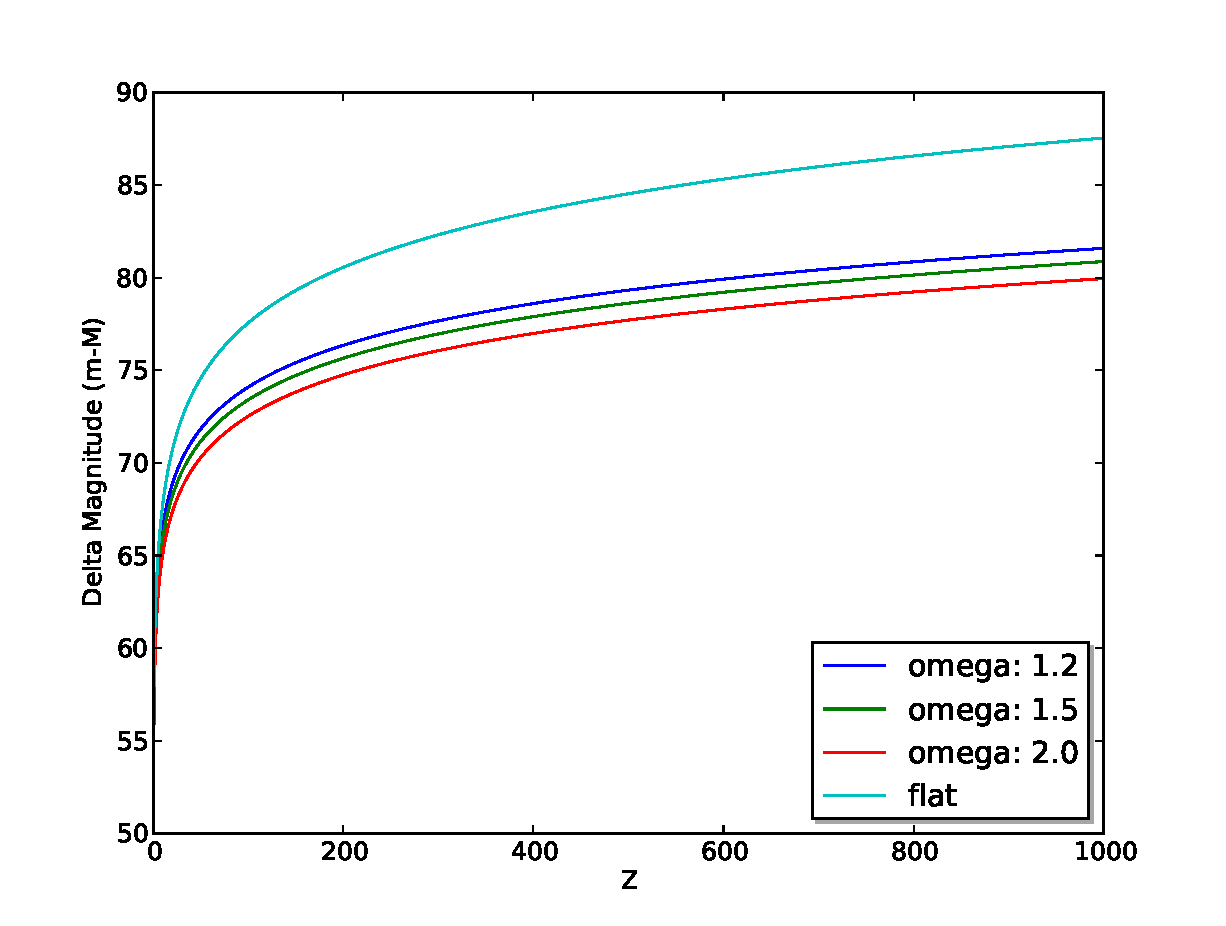
\includegraphics[scale=.6]{plot_2.pdf}
\caption{$\Delta$ magnitude vs redshift for a flat matter dominated universe with $H_0=70km/s/Mpc$ and for a matter dominated closed universe with $\Omega_m=1.2,1.5,2$}
\end{center}
\end{figure}

\end{document}
